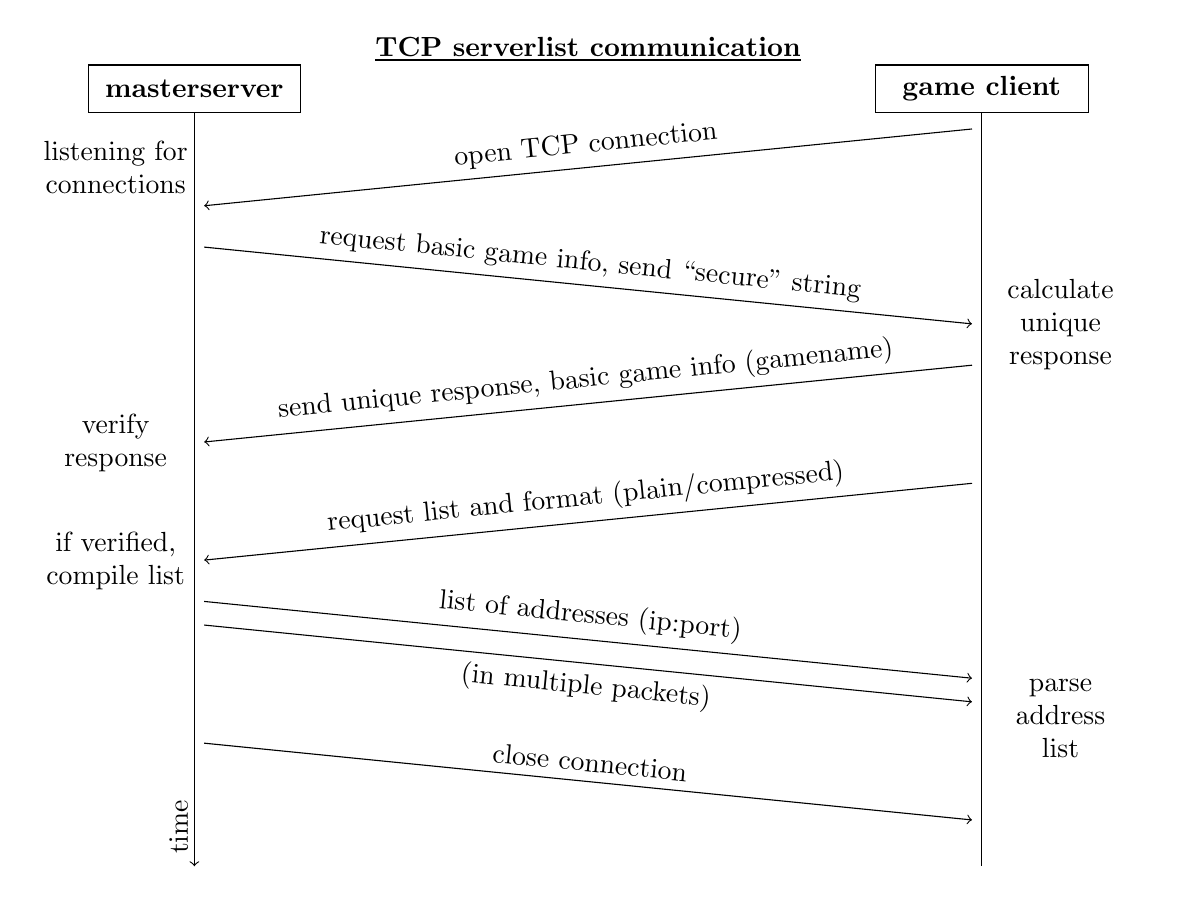
\begin{tikzpicture}

% figure title
\node[rectangle] at (5, 10.5) (title) {\underline{\bf TCP serverlist communication}};

% ms and gc, top
\node[draw, rectangle, minimum height=0.6cm, minimum width=2.7cm] at (0,  10.0) (mstop) {\bf masterserver};
\node[draw, rectangle, minimum height=0.6cm, minimum width=2.7cm] at (10, 10.0) (gctop) {\bf game client};

% open connection
\node at (10,  9.5) (gcoc) {};
\node at ( 0,  8.5) (msoc) {};
\node at (-1,  9.0) (mslisten) [text width=2cm, text centered]{listening for\\connections};
\draw[->] (gcoc) -- (msoc) node[midway, above, sloped] {open TCP connection};

% secure
\node at ( 0,  8.0) (msse) {};
\node at (10,  7.0) (gcse) {};
\node at (11,  7.0) (gcsecure) [text width=2cm,text centered]{calculate unique\\ response};
\draw[->] (msse) -- (gcse) node[midway, above, sloped] {request basic game info, send ``secure'' string};

% validate        
\node at (10,  6.5) (gcva) {};
\node at ( 0,  5.5) (msva) {};
\node at (-1,  5.5) (msvalidate) [text width=2cm,text centered]{verify\\ response};
\draw[->] (gcva) -- (msva) node[midway, above, sloped] {send unique response, basic game info (gamename)};

% list request
\node at (10,  5.0) (gcli) {};
\node at ( 0,  4.0) (msli) {};
\node at (-1,  4.0) (mslist) [text width=2cm, text centered]{if verified, compile list};
\draw[->] (gcli) -- (msli) node[midway, above, sloped] {request list and format (plain/compressed)};

\node at ( 0,  3.5) (msl1) {};
\node at (10,  2.5) (gcl1) {};
\draw[->] (msl1) -- (gcl1) node[midway, above, sloped] {list of addresses (ip:port)};

\node at ( 0,  3.2) (msl2) {};
\node at (10,  2.2) (gcl2) {};
\node at (11,  2.0) (gcparse) [text width=2cm, text centered]{parse\\address\\list};
\draw[->] (msl2) -- (gcl2) node[midway, below, sloped] {(in multiple packets)};

% close connection
\node at ( 0,  1.7) (mscc) {};    
\node at (10,  0.7) (gccc) {};    
\draw[->] (mscc) -- (gccc) node[midway, above, sloped] {close connection};

% ms and gc, bottom, vertical lines
\node at ( 0, 0) (msbot) {};
\node at (10,  0.0) (gcbot) {};
\draw[->] (mstop.270) -- (msbot.90) node[at end, xshift=-0.2cm, yshift=0.5cm, rotate=90] {time};
\draw (gctop.270) -- (gcbot.90) {};

\end{tikzpicture}
